
\subsection{Face Recognition dengan video}
\begin{enumerate}[1.]
\item Proses mengumpulkan dataset dengan video

- Memasukan library openCV, yaitu \textbf{cv2}
\begin{figure}[h!]
    \centering
    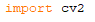
\includegraphics[width=0.3\linewidth]{images/fr_1.PNG}
    \caption{Memasukan library openCV}
\end{figure}

-  Proses face detection, untuk melakukan proses deteksi wajah akan menggunakan algoritma \emph{haarcascade}. Dengan fungsi \textbf{cv2.CascadeClassifier} pada baris pertama, 
pada baris kedua merupakan fungsi openCV untuk memasukan video atau kamera yang terhubung dengan \textbf{cv2.VideoCapture()}
\begin{figure}[h!]
    \centering
    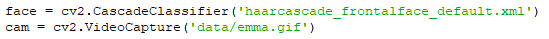
\includegraphics[width=0.85\linewidth]{images/fr_2.PNG}
    \caption{Proses face detection dengan masukan video}
\end{figure}\\

- Menambahkan variabel 'jumlah' yang dimulai dari 0 untuk menyimpan data perulangan pengambilan gambar dataset
dan juga pada baris selanjutnya ada variabel 'id' wadah masukan user untuk id dataset
\begin{figure}[h!]
    \centering
    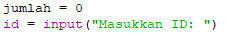
\includegraphics[width=0.45\linewidth]{images/fr_3.PNG}
    \caption{Tambah variabel}
\end{figure}
\newpage
- Membaca video atau kamera yang sudah dimasukkan sebelumnya dengan fungsi \textbf{read()}, dan untuk mengubah warna citra menjasi hitam-putih/grayscale
dengan fungsi \textbf{cv2.cvtColor}
\begin{figure}[h!]
    \centering
    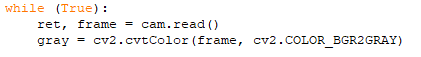
\includegraphics[width=0.85\linewidth]{images/fr_4.PNG}
    \caption{Membaca video dan merubah warna citra}
\end{figure}

- Pada baris pertama fungsi untuk deteksi wajah dengan fungsi \textbf{detectMultiScale()}. 
Pada baris selanjutnya ada fungsi membuat bingkai \textbf{cv2.rectangle} lalu ada pengulangan untuk jumlah gambar yang ditangkap
, lalu ada \textbf{cv2.imwrite} untuk menyimpan gambar data direktori dataset yang telah ditentukan, dan \textbf{cv2.imshow} untuk 
menampilkan video atau kamera yang aka dideteksi dan diambil gambar untuk dataset.
\begin{figure}[h!]
    \centering
    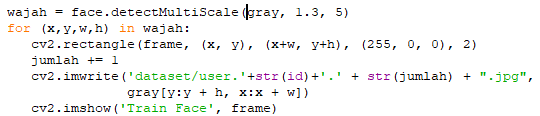
\includegraphics[width=0.85\linewidth]{images/fr_5.PNG}
    \caption{Penyimpanan dataset}
\end{figure}

- Menentukan jumlah gambar yang akan tersimpan pada dataset
\begin{figure}[h!]
    \centering
    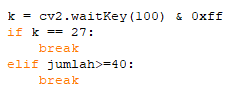
\includegraphics[width=0.5\linewidth]{images/fr_6.PNG}
    \caption{Mengatur jumlah gambar yang diambil}
\end{figure}
\newpage
- Keseluruhan kode program untuk pengambilan dataset
\begin{figure}[h!]
    \centering
    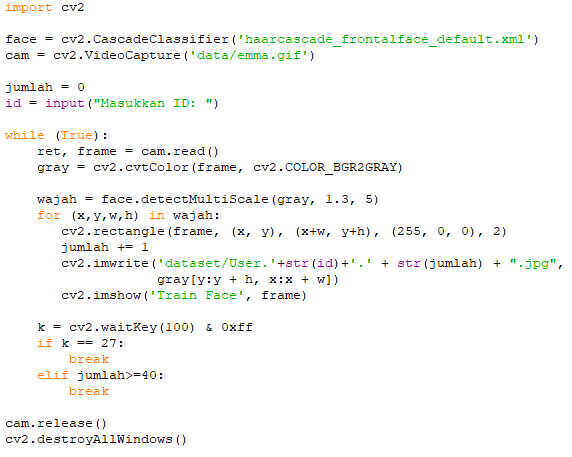
\includegraphics[width=0.85\linewidth]{images/fr_full.PNG}
    \caption{Kode pengambilan dataset}
\end{figure}

- Percobaan pengambilan dataset untuk tiga ID menggunakan masukan video
\begin{figure}[h!]
    \centering
    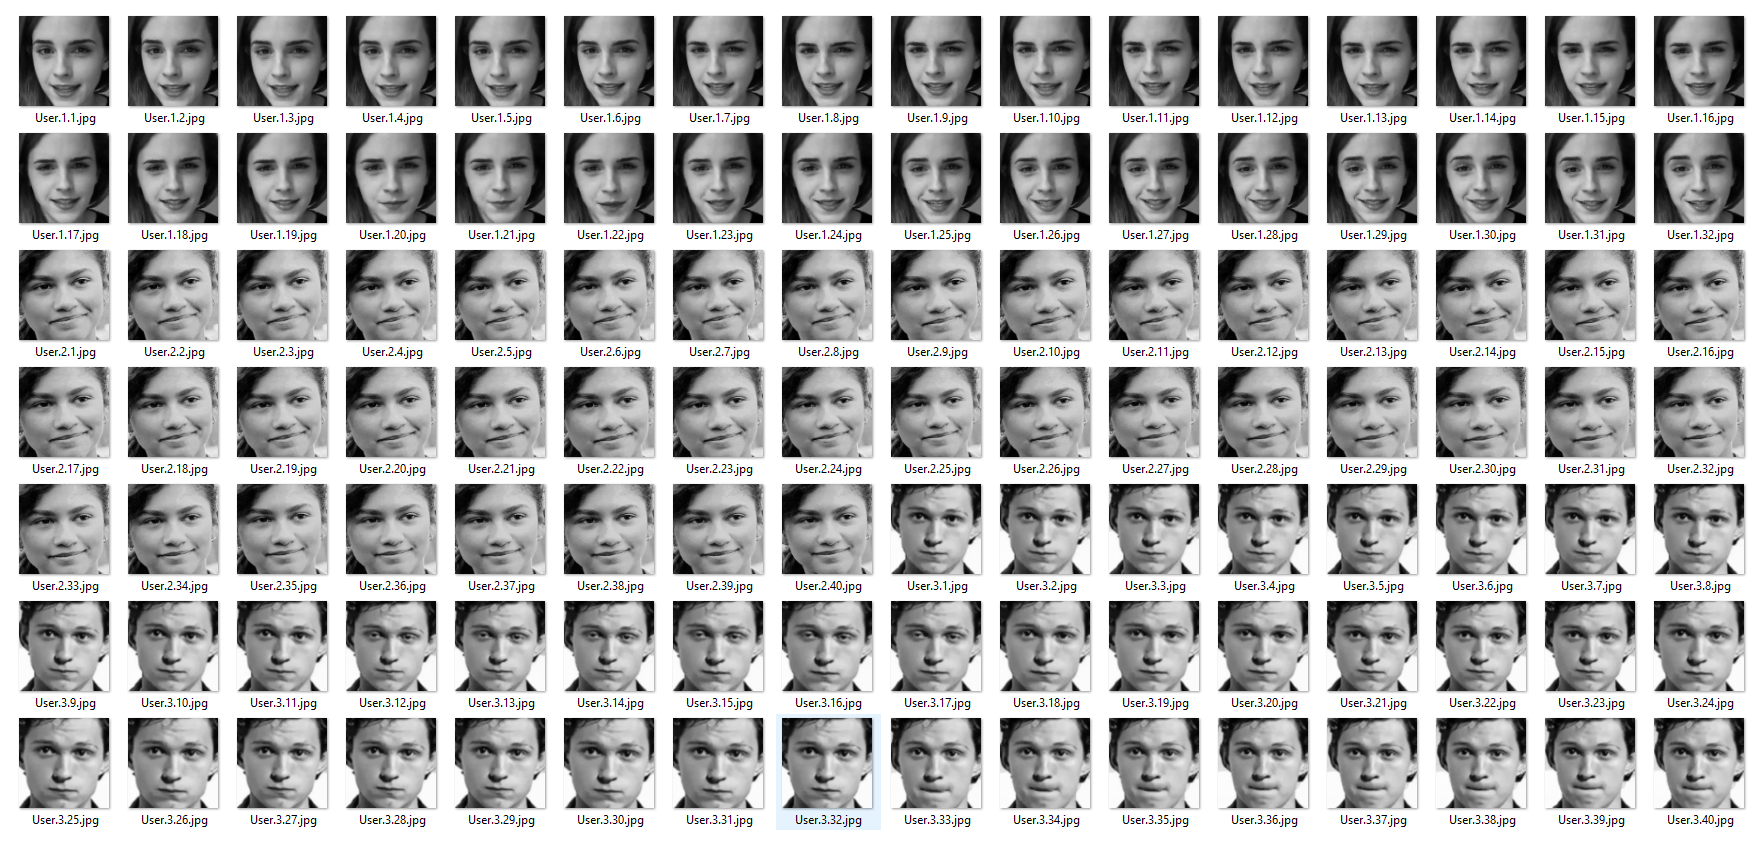
\includegraphics[width=1.2\linewidth]{images/dataset.PNG}
    \caption{Pengambilan dataset}
\end{figure}

\item Proses training dataset

- Import library cv2, numpy, Image from PIL (Pillow) library, dan os
\begin{figure}[h!]
    \centering
    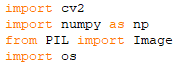
\includegraphics[width=0.4\linewidth]{images/train_1.PNG}
    \caption{Pengambilan dataset}
\end{figure}

- pada baris ke-1, memasukan nama direktori dataset pada variabel path 

Pada baris ke-2, untuk pengenalan wajah, menggunakan model algoritma LBPH yang sudah tersedia pada openCV

Pada bari ke-3,  Proses face detection, untuk melakukan proses deteksi wajah akan menggunakan algoritma haarcascade
\begin{figure}[h!]
    \centering
    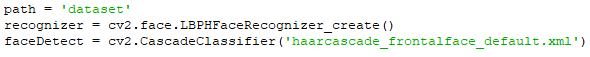
\includegraphics[width=0.9\linewidth]{images/train_2.PNG}
    \caption{Pengambilan dataset}
\end{figure}

- Membuat method atau fungsi untuk mendapatkan image dataset sebagai data training agar dikenali oleh bahasa komputer
\begin{figure}[h!]
    \centering
    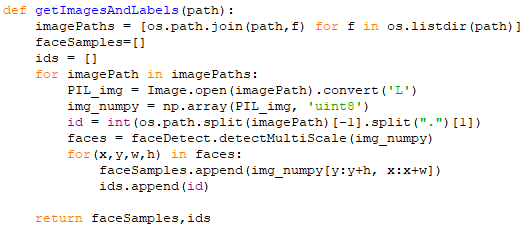
\includegraphics[width=0.9\linewidth]{images/train_3.PNG}
    \caption{Pengambilan dataset}
\end{figure}\\
Memasukan direktori dataset pada variabel path menggunakan \textbf{os.path.join()} kedalam variabel imagePath.
Lalu kumpulan image training akan diubah menggunakan library PIL menjadi sebuah array. Setelah itu, array data training akan dibuat oleh numpy.
Dimana array yang diambil merupakan id dan juga faceSample.
\newpage
- Training data
\begin{figure}[h!]
    \centering
    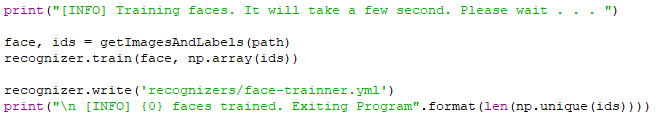
\includegraphics[width=0.9\linewidth]{images/train_4.PNG}
    \caption{Pengambilan dataset}
\end{figure}\\
Fungsi "getImagesAndLabels (path)", akan mengambil semua foto di direktori: "dataset/", mengembalikan 2 array: "Ids" dan "faces". 
Dengan array tersebut sebagai input, data akan di training menggunakan fungsi \textbf{recognizer.train()}
Untuk hasil training data akan disimpan dalam bentuk \textbf{.yml} pada direktori recognizers dengan fungsi \textbf{recognizer.write()}

- Proses training data
\begin{figure}[h!]
    \centering
    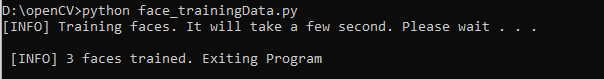
\includegraphics[width=0.9\linewidth]{images/train_data.PNG}
    \caption{Pengambilan dataset}
\end{figure}

- Hasil training data berbentuk file \textbf{.yml}
\begin{figure}[h!]
    \centering
    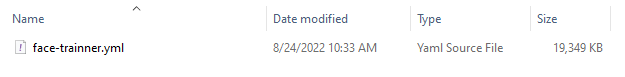
\includegraphics[width=1\linewidth]{images/hasil_train.PNG}
    \caption{Pengambilan dataset}
\end{figure}

\item Proses pengenalan wajah

- Import library, dengan menggunakan library numpy, cv2, dan juga os
\begin{figure}[h!]
    \centering
    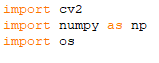
\includegraphics[width=0.45\linewidth]{images/recognition_1.PNG}
    \caption{Import Library}
\end{figure}
\newpage
- Melakukan pengenalan wajah menggunakan algoritman LBPH pada variabel \textbf{recognizer}, selanjutnya variabel recognizer 
membaca hasil dari training dataset dalam bentuk file \textbf{.yml} untuk mengekstrak data yang ada di dalam file 
\begin{figure}[h!]
    \centering
    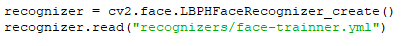
\includegraphics[width=0.75\linewidth]{images/recognition_2.PNG}
    \caption{Pengenalan wajah}
\end{figure}

- Proses deteksi wajah untuk dilakukan pengenalan/pencocokan wajah menggunakan algoritma \emph{Haar-Cascade Classifier}
\begin{figure}[h!]
    \centering
    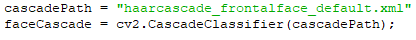
\includegraphics[width=0.75\linewidth]{images/recognition_3.PNG}
    \caption{Deteksi wajah}
\end{figure}

- Baris untuk tipe font yang akan diunculkan, serta variabel id untuk menampung id dataset
\begin{figure}[h!]
    \centering
    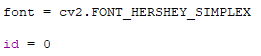
\includegraphics[width=0.5\linewidth]{images/recognition_4.PNG}
    \caption{Font dan ID}
\end{figure}

- Pembuatan array baru untuk menampilkan nama sesuai id 
\begin{figure}[h!]
    \centering
    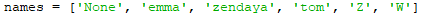
\includegraphics[width=0.75\linewidth]{images/recognition_5.PNG}
    \caption{Array nama}
\end{figure}

- Proses memasukan video atau device kamera, dan untuk mengatur ukuran frame yang akan ditampilkan
\begin{figure}[h!]
    \centering
    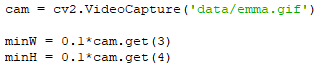
\includegraphics[width=0.75\linewidth]{images/recognition_6.PNG}
    \caption{Input video/kamera serta mengatur ukuran frame}
\end{figure}
\newpage
- Untuk membaca video atau kamera yang dimasukkan sebelumnya, lalu mengubah warna menjadi grayscal. 
Kemudian deteksi gambar menggunakan \textbf{detecMultiScale()}
\begin{figure}[h!]
    \centering
    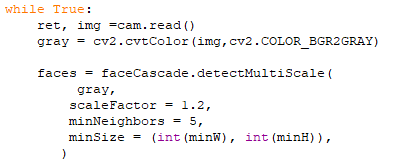
\includegraphics[width=0.7\linewidth]{images/recognition_7.PNG}
    \caption{Membaca dan perubahan citra}
\end{figure}

- \textbf{recognizer.predict()}, akan mengambil sebagai parameter bagian 
wajah yang ditangkap untuk dianalisis kecocokannya dengan data training dan akan mengembalikan kemungkinan kecocokan data
\begin{figure}[h!]
    \centering
    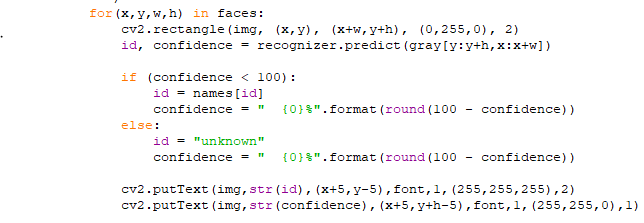
\includegraphics[width=1\linewidth]{images/recognition_8.PNG}
    \caption{Mengenali kecocokan data}
\end{figure}\\
untuk kondisi \textbf{if else} untuk mengatur tampilnya data jika ada kecocokan dalam bentuk persentase.
Jika ada kecocokan akan ditampilkan id yang sudah diganti dengan nama pada array dan juga besaran presentase 
yang dikenali oleh recognitor.

- Proses menampilkan video/kamera dan juga fungsi \textbf{waitKey()} untuk menutup program jika mekan tombol 'ESC'
\begin{figure}[h!]
    \centering
    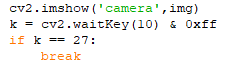
\includegraphics[width=0.45\linewidth]{images/recognition_9.PNG}
    \caption{Menampilkan kamera atau video serta akhir program}
\end{figure}
\newpage
- Hasil recognition dengan masukan video dan pembuatan label nama
\begin{figure}[h!]
    \centering
    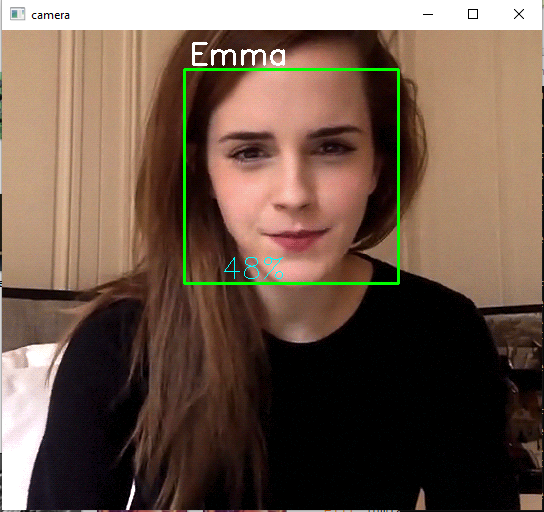
\includegraphics[width=0.65\linewidth]{images/Hasil_recog.PNG}
    \caption{Hasil recognition video}
\end{figure}
\end{enumerate}